\documentclass[11pt]{article}
    %	options include 12pt or 11pt or 10pt
    %	classes include article, report, book, letter, thesis
    
    \title{HW1}
    \author{Shane Drafahl}
    \date{29 August,2017}
    \usepackage{graphicx}
    \usepackage{epstopdf}

    \begin{document}
    \maketitle

    1. Give a regular expression, simplified to the best of your abilities, for the language of all strings
    of a’s, b’s, and c’s where a is never immediately followed by b.
    $ \newline \newline $
    $ \sum $ = $ \{\ a, b, c \}\ $
    $ \newline \newline $
    $ ((a + c)^{*}(c^{+}b^{*})^{*}(a + c)^{*})^{*} $ + $ ((a^{*}c^{+})^{*}(b^{*})^{*}((a^{*}c^{+})^{*})^{*} $
    
    $ \newline $

    2. Give a regular expression, simplified to the best of your abilities, for the language of all strings
    of a’s, b’s, and c’s that contain an even number of b’s.

    $ \newline $

    $ \sum $ = $ \{\ a, b, c \}\ $
    $ \newline \newline $
    $ (a + c)^{*} + ((a + c)^{*} b (a + c)^{*}b)^{*} $
    
    $ \newline $

    3. Simplify (if possible) the expression $ (a + b + c)^{*}(a + b)^{*} $ , 
    then describe as concisely as you can in English the language it defines.

    $ \newline $
    
    This regular expression is equal to $(a^{*}b^{*}c^{*})^{*} (a^{*} b^{*})^{*} $ and be reduced to
    $ (a + b + c)^{*} $. In english it essentialy means that the language created from it
    has a general form of a-b-c and this form can repeat with repeating letters such as
    aaa-bbb-cc-aa-bb-cc.

    $ \newline $

    4. Simplify (if possible) the expression $(a + b)^{*}c^{*}(a + b)^{*}$ , then describe as concisely as you can
    in English the language it defines.

    $ \newline $

    This could be simplified/converted to $ (a^{*}b^{*})^{*}c^{*}(a^{*}b^{*})^{*} $. In english it essentialy
    means a language of the form where a-b-c-a-b where there is a number of c's or none in the middle 
    but on the outside there is a pattern of a-b where they can repeat the characters and the the pattern
    such as aa-bb-aa-bb in that order.

    $ \newline $

    5. Define a DFA, simplified to the best of your abilities, for the language of all strings of a’s,
    b’s, and c’s where a is never immediately followed by b.

    \begin{figure}[!htb]
        \centering
        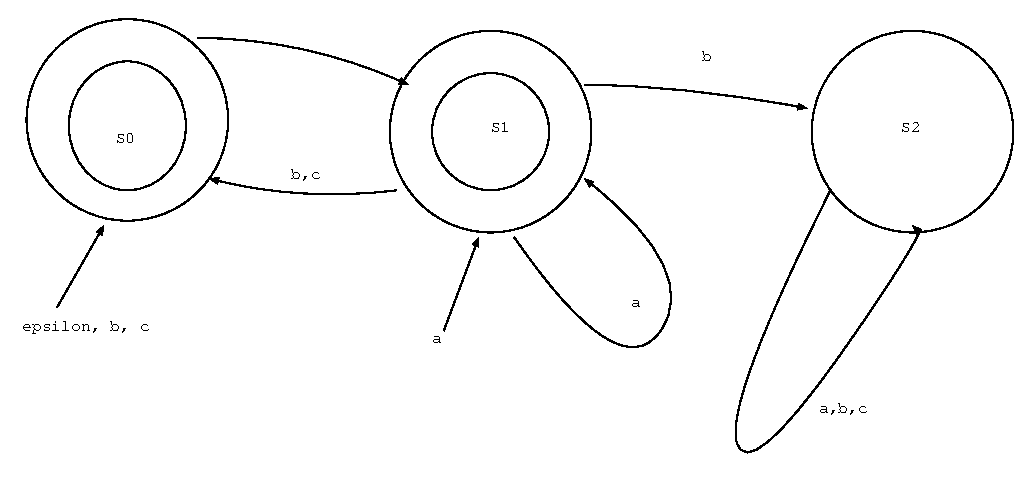
\includegraphics[scale=.7]{hw1_1.eps}
    \end{figure}

    $ \newline $

    6. Define a DFA, simplified to the best of your abilities, that recognizes the language

    \begin{figure}[!htb]
        \centering
        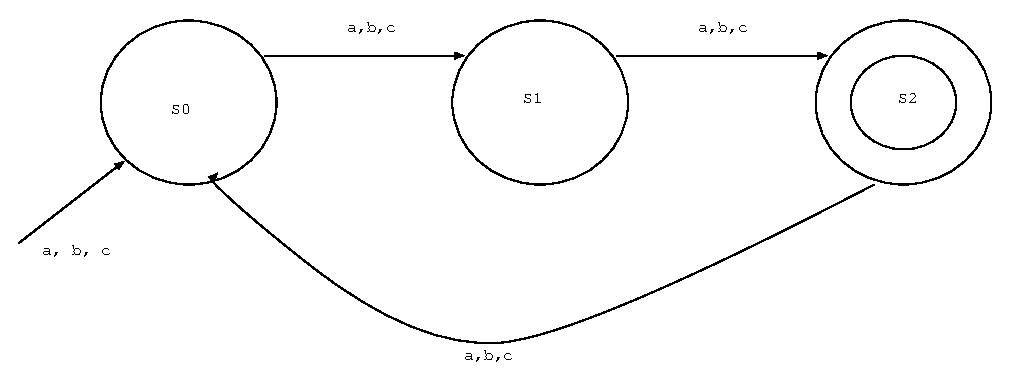
\includegraphics[scale=.7]{hw1_2.eps}
    \end{figure}

    $ \newline \newline $

    

    \end{document}
    